\documentclass[
  jou,
  longtable,
  colorlinks=true,linkcolor=blue,citecolor=blue,urlcolor=blue]{apa7}


\ifLuaTeX
\usepackage[bidi=basic]{babel}
\else
\usepackage[bidi=default]{babel}
\fi
\babelprovide[main,import]{english}


% get rid of language-specific shorthands (see #6817):
\let\LanguageShortHands\languageshorthands
\def\languageshorthands#1{}

\RequirePackage{longtable}
% \setlength\LTleft{0pt}
\RequirePackage{threeparttablex}

% % % 
% % 


\makeatletter
\renewcommand{\paragraph}{\@startsection{paragraph}{4}{\parindent}%
	{0\baselineskip \@plus 0.2ex \@minus 0.2ex}%
	{-.5em}%
	{\normalfont\normalsize\bfseries\typesectitle}}

\renewcommand{\subparagraph}[1]{\@startsection{subparagraph}{5}{0.5em}%
	{0\baselineskip \@plus 0.2ex \@minus 0.2ex}%
	{-\z@\relax}%
	{\normalfont\normalsize\bfseries\itshape\hspace{\parindent}{#1}\textit{\addperi}}{\relax}}
\makeatother

\usepackage{amsmath}


\usepackage{longtable, booktabs, multirow, multicol, colortbl, hhline, caption, array, float}
\setcounter{topnumber}{2}
\setcounter{bottomnumber}{2}
\setcounter{totalnumber}{4}
\renewcommand{\topfraction}{0.85}
\renewcommand{\bottomfraction}{0.85}
\renewcommand{\textfraction}{0.15}
\renewcommand{\floatpagefraction}{0.7}

\usepackage{tcolorbox}
\tcbuselibrary{listings,theorems, breakable, skins}
\usepackage{fontawesome5}

\definecolor{quarto-callout-color}{HTML}{909090}
\definecolor{quarto-callout-note-color}{HTML}{0758E5}
\definecolor{quarto-callout-important-color}{HTML}{CC1914}
\definecolor{quarto-callout-warning-color}{HTML}{EB9113}
\definecolor{quarto-callout-tip-color}{HTML}{00A047}
\definecolor{quarto-callout-caution-color}{HTML}{FC5300}
\definecolor{quarto-callout-color-frame}{HTML}{ACACAC}
\definecolor{quarto-callout-note-color-frame}{HTML}{4582EC}
\definecolor{quarto-callout-important-color-frame}{HTML}{D9534F}
\definecolor{quarto-callout-warning-color-frame}{HTML}{F0AD4E}
\definecolor{quarto-callout-tip-color-frame}{HTML}{02B875}
\definecolor{quarto-callout-caution-color-frame}{HTML}{FD7E14}


% 

\newlength\Oldarrayrulewidth
\newlength\Oldtabcolsep


\usepackage{hyperref}




\providecommand{\tightlist}{%
  \setlength{\itemsep}{0pt}\setlength{\parskip}{0pt}}
\usepackage{longtable,booktabs,array}
\usepackage{calc} % for calculating minipage widths
% Correct order of tables after \paragraph or \subparagraph
\usepackage{etoolbox}
\makeatletter
\patchcmd\longtable{\par}{\if@noskipsec\mbox{}\fi\par}{}{}
\makeatother
% Allow footnotes in longtable head/foot
\IfFileExists{footnotehyper.sty}{\usepackage{footnotehyper}}{\usepackage{footnote}}
\makesavenoteenv{longtable}

\usepackage{graphicx}
\makeatletter
\def\maxwidth{\ifdim\Gin@nat@width>\linewidth\linewidth\else\Gin@nat@width\fi}
\def\maxheight{\ifdim\Gin@nat@height>\textheight\textheight\else\Gin@nat@height\fi}
\makeatother
% Scale images if necessary, so that they will not overflow the page
% margins by default, and it is still possible to overwrite the defaults
% using explicit options in \includegraphics[width, height, ...]{}
\setkeys{Gin}{width=\maxwidth,height=\maxheight,keepaspectratio}
% Set default figure placement to htbp
\makeatletter
\def\fps@figure{htbp}
\makeatother


% definitions for citeproc citations
\NewDocumentCommand\citeproctext{}{}
\NewDocumentCommand\citeproc{mm}{%
  \begingroup\def\citeproctext{#2}\cite{#1}\endgroup}
\makeatletter
 % allow citations to break across lines
 \let\@cite@ofmt\@firstofone
 % avoid brackets around text for \cite:
 \def\@biblabel#1{}
 \def\@cite#1#2{{#1\if@tempswa , #2\fi}}
\makeatother
\newlength{\cslhangindent}
\setlength{\cslhangindent}{1.5em}
\newlength{\csllabelwidth}
\setlength{\csllabelwidth}{3em}
\newenvironment{CSLReferences}[2] % #1 hanging-indent, #2 entry-spacing
 {\begin{list}{}{%
  \setlength{\itemindent}{0pt}
  \setlength{\leftmargin}{0pt}
  \setlength{\parsep}{0pt}
  % turn on hanging indent if param 1 is 1
  \ifodd #1
   \setlength{\leftmargin}{\cslhangindent}
   \setlength{\itemindent}{-1\cslhangindent}
  \fi
  % set entry spacing
  \setlength{\itemsep}{#2\baselineskip}}}
 {\end{list}}
\usepackage{calc}
\newcommand{\CSLBlock}[1]{\hfill\break\parbox[t]{\linewidth}{\strut\ignorespaces#1\strut}}
\newcommand{\CSLLeftMargin}[1]{\parbox[t]{\csllabelwidth}{\strut#1\strut}}
\newcommand{\CSLRightInline}[1]{\parbox[t]{\linewidth - \csllabelwidth}{\strut#1\strut}}
\newcommand{\CSLIndent}[1]{\hspace{\cslhangindent}#1}


\usepackage{times}
    


\title{\vskip 1.5cm
\bfseries Acute Beetroot Supplementation May Improve Blood Pressure \\ but not Exercise Economy in Female Masters Swimmers}
\shorttitle{Template for the apaquarto Extension}


\usepackage{etoolbox}


\journal{\bfseries \Large Journal of Kinesiology and Wellness}
\volume{\vskip 1mm \normalsize A Publication of the Western Society for
Kinesiology and Wellness \newline Volume 12, Number 1, Pages 1--9,
2023\newline ISSN\# 2323-4505}




\authorsnames[{1},{1},{2,3},{4}]{
Ana Fulano,Blanca Zutano,Carina Mengano,Dolorita Perengano
}



\authorsaffiliations{
{Department of Psychology, Ana and Blanca's University},{Carina's
Primary Affiliation},{Carina's Secondary Affiliation},{Buffalo, NY }}






\leftheader{Fulano, Zutano, Mengano and Perengano}



\abstract{This document is a template demonstrating the apaquarto
format. This document is a template demonstrating the apaquarto
format.This document is a template demonstrating the apaquarto format.
This document is a template demonstrating the apaquarto format. This
document is a template demonstrating the apaquarto format. This document
is a template demonstrating the apaquarto format. This document is a
template demonstrating the apaquarto format. This document is a template
demonstrating the apaquarto format. This document is a template
demonstrating the apaquarto format. This document is a template
demonstrating the apaquarto format. This document is a template
demonstrating the apaquarto format. This document is a template
demonstrating the apaquarto format. This document is a template
demonstrating the apaquarto format.}
% 
\keywords{keyword1, keyword2, keyword3}

\authornote{\par{\addORCIDlink{Ana
Fulano}{0000-0000-0000-0001}}\par{\addORCIDlink{Blanca
Zutano}{0000-0000-0000-0002}}\par{\addORCIDlink{Carina
Mengano}{0000-0000-0000-0003}}\par{\addORCIDlink{Dolorita
Perengano}{0000-0000-0000-0004}}
\par{ }
\par{       Author roles were classified using the Contributor Role Taxonomy (CRediT; https://credit.niso.org/) as follows: Ana
Fulano:   conceptualization, writing; Blanca Zutano:   project
administration, formal analysis; Carina Mengano:   formal
analysis, writing; Dolorita Perengano:   writing, methodology, formal
analysis}
\par{Correspondence concerning this article should be addressed to Ana
Fulano, Department of Psychology, Ana and Blanca's University, 1234
Capital St., Albany, NY 12084-1234, Email: sm@example.org}
}


\usepackage{float}
\makeatletter
\let\oldtpt\ThreePartTable
\let\endoldtpt\endThreePartTable
\def\ThreePartTable{\@ifnextchar[\ThreePartTable@i \ThreePartTable@ii}
\def\ThreePartTable@i[#1]{\begin{figure}
\onecolumn
\begin{minipage}{0.5\textwidth}
\oldtpt[#1]
}
\def\ThreePartTable@ii{\begin{figure}
\onecolumn
\begin{minipage}{0.5\textwidth}
\oldtpt
}
\def\endThreePartTable{
\endoldtpt
\end{minipage}
\twocolumn
\end{figure}}
\makeatother


\makeatletter
\let\endoldlt\endlongtable		
\def\endlongtable{
\hline
\endoldlt}
\makeatother

\newenvironment{twocolumntable}% environment name
{% begin code
\begin{table*}%
\onecolumn%
}%
{%
\twocolumn%
\end{table*}%
}% end code

\urlstyle{same}





\begin{document}
\maketitle
\setcounter{secnumdepth}{-\maxdimen} % remove section numbering

\setlength\LTleft{0pt}


Weight bias (i.e., anti-fat bias) is unreasonable judgments about
someone based on weight (Washington, 2011). It is pervasive in the
health industry, including those who work as physicians (Schwartz et
al., 2003), physical educators (Fontana et al., 2017), fitness
professionals (Dimmock et al., 2009; Fontana et al., 2018; Robertson \&
Vohora, 2008), and exercise science students (Chambliss et al., 2004;
Fontana et al., 2013; Langdon et al., 2016; Rukavina et al., 2010;
Wijayatunga et al., 2019). In the fitness industry, potential
implications of these biases include negative perceptions of larger
bodied individuals' abilities, motivation, and potential job
qualifications (Sartore \& Cunningham, 2007). Weight stigma is defined
as discriminatory acts towards individuals in larger bodies due to their
size (Washington, 2011). Consequences of experiencing weight stigma
include a) poor physical health, such as an increased likelihood of
maintained obesity or weight gain (Sutin \& Terracciano, 2013), and b)
increased psychological distress, including greater rates of body
dissatisfaction and symptoms of eating disorders (Vartanian \& Novak,
2011). Paradoxically, individuals who experience weight stigma are more
likely to avoid exercise as a result of internalized anti-fat attitudes
(Vartanian \& Novak, 2011) and experience an increased allostatic load
(cumulative response to ongoing stress) (Guidi et al., 2021), which has
a greater impact on their health than being in a larger body does
(Gordon, 2020; Milburn et al., 2019).

A systematic review on weight bias among exercise and nutrition
professionals included 31 studies; however, only three focused
specifically on fitness professionals (e.g., personal trainers or group
fitness instructors) compared to ``exercise professional trainees''
(e.g., exercise science students). Robertson and Vohora (2008) were the
first to report strong anti-fat implicit and explicit biases in fitness
professionals (n = 57, ``gym instructors'' and ``aerobics
instructors''), with the bias being greater in those who had never been
overweight and believed obesity was controllable. In a study surveying
fitness center employees (management and administrative staff n = 15,
personal trainers n = 16, fitness instructors n =19, and exercise/sport
physiologists n = 20), Dimmock et al.~(2009) reported a moderately
strong implicit bias, but no explicit bias, towards individuals in
larger body sizes. More recently, Fontana et al.~(2018) found that
personal trainers (n = 52) report strong implicit biases against
individuals who are obese.

Recently, Zaroubi et al.~(2021) published a review article on the
predictors of weight bias in fitness professionals and exercise science
students (Zaroubi et al., 2021). Most of the studies in this review
sampled undergraduate students in the exercise science field, with only
four of the 18 sample fitness professionals. Of those four studies, only
three included weight bias as a dependent variable (Dimmock et al.,
2009; Fontana et al., 2018; Robertson \& Vohora, 2008). A thematic
analysis was conducted, and six themes emerged. First, exercise science
students and fitness professionals strongly believe that weight is
controllable and associate individuals with larger bodies with negative
attributes such as laziness. Second, the relationship between gender and
weight bias is still unknown as data is conflicting. Third, being
enrolled in an exercise science or similar educational program is likely
a predictor of weight bias. Fourth, personal and psychosocial factors
(e.g., the tendency to internalize an athletic body as the ideal body
shape) likely influence weight bias. Fifth, knowledge of the
uncontrollable aspects of obesity (e.g., genetics) is likely to lower
weight bias. Lastly, there is conflicting evidence regarding the
influence of one's personal history with someone in a larger body.
Chambliss et al.~(2004) report that a lack of family history of having a
larger body leads to higher explicit weight bias in fitness
professionals and regular exercisers (Chambliss et al., 2004). In
contrast, DeBarr and Pettit reported no statistical differences in
weight bias held by health educators classified as overweight compared
to normal weight.

Little research has examined explicit weight biases of fitness
professionals, and no research has focused on whether their social
identities and/or role in the industry (e.g., group fitness instructor
versus personal trainer) influence their weight bias. This research is
particularly important due to the influential nature of this field.
Clients often look to fitness professionals for advice and education on
changing their health behaviors. If fitness professionals hold strong
weight biases, they may contribute to a harmful cycle whereby their
clients become less likely to participate and/or adhere to their health
behavior changes. Fitness professionals need to have more knowledge of
weight biases. Thus, the study aimed to examine the influence of age,
gender, body dissatisfaction, race, role in industry, BMI, income, and
education on weight bias in fitness professionals.

\section{Results}\label{results}

There was a statistically significant interaction between gender and BMI
on total AFAT scores, F(2,272) = 3.139, p = .045, partial 2 = .023.
Therefore, an analysis of simple main effects for gender and BMI was
performed with statistical significance receiving a Bonferroni
adjustment. Women in the healthy (2.02  .51) and overweight (1.97 
.49) BMI categories had significantly greater total AFAT scores (p =
.003 and p = .023, respectively) compared to women in the obese BMI
category (1.63  .48). There was also a statically significant
interaction between education and BMI on total AFAT scores, F(9,266) =
2.201, p = .022, partial 2 = .069. An analysis of simple main effects
for education and BMI was performed with statistical significance
receiving a Bonferroni adjustment. For participants who had completed
some college, those who were classified in the healthy BMI category had
significantly greater total AFAT scores (2.05  .50) compared to those
in the overweight BMI category (1.72  .46), p = .045. For participants
who completed a master's degree, those in the healthy BMI category (2.08
 .56) and overweight BMI category (2.05  .43) had significantly
greater total AFAT scores (p = .003 and .016, respectively) compared to
those in the obese BMI category (1.48  .46). No other interaction
effects were found. Therefore, one-way ANOVAs and MANOVAs were conducted
to assess the direct effect of the IVs on AFAT total and AFAT subscales,
respectively. The mean total AFAT scores for each IV are listed in Table
7.

\subsection{Age}\label{age}

rrr

\subsection{Displaying Figures}\label{displaying-figures}

A reference label for a figure must have the prefix \texttt{fig-}, and
in a code chunk, the caption must be set with \texttt{fig-cap}. Captions
are in
\href{https://apastyle.apa.org/style-grammar-guidelines/capitalization/title-case}{title
case}.

\begin{figure}[!htbp]

{\caption{{The Figure Caption}{\label{fig-myplot}}}}

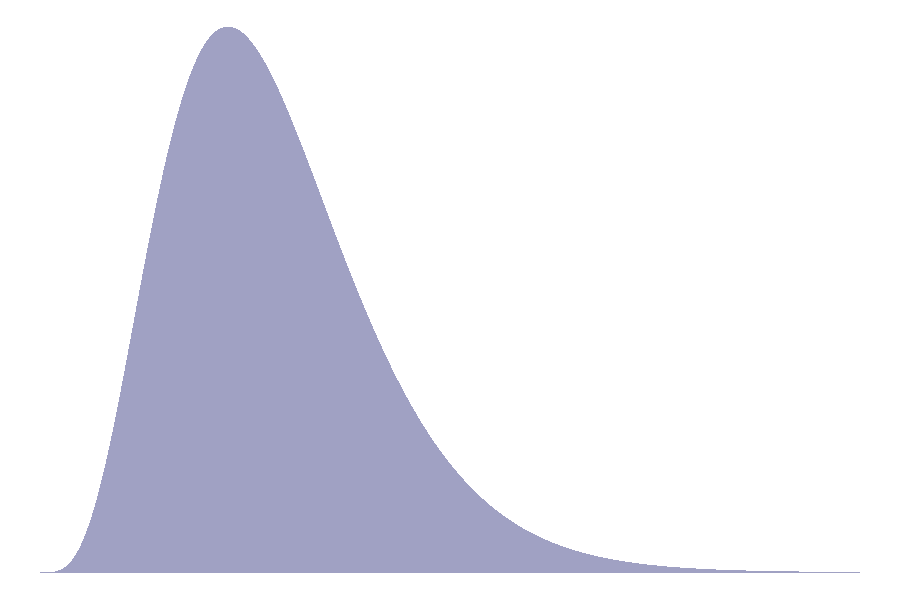
\includegraphics{modi_golnick_files/figure-pdf/fig-myplot-1.pdf}

{\noindent \emph{Note.} This is the note below the figure.}

\end{figure}

To refer to any figure or table, use the \texttt{@} symbol followed by
the reference label (e.g., Figure~\ref{fig-myplot}).

\subsection{Imported Graphics}\label{imported-graphics}

One way to import an existing graphic as a figure is to use
\texttt{knitr::include\_graphics} in a code chunk. For example,
Figure~\ref{fig-import1} is an imported image. Note that in
apaquarto-pdf documents, we can specify that that a figure or table
should span both columns when in journal mode by setting the
\texttt{apa-twocolumn} chunk option to \texttt{true}. For other formats,
this distinction does not matter.

\begin{figure*}[!htbp]

{\caption{{An Imported Graphic}{\label{fig-import1}}}}

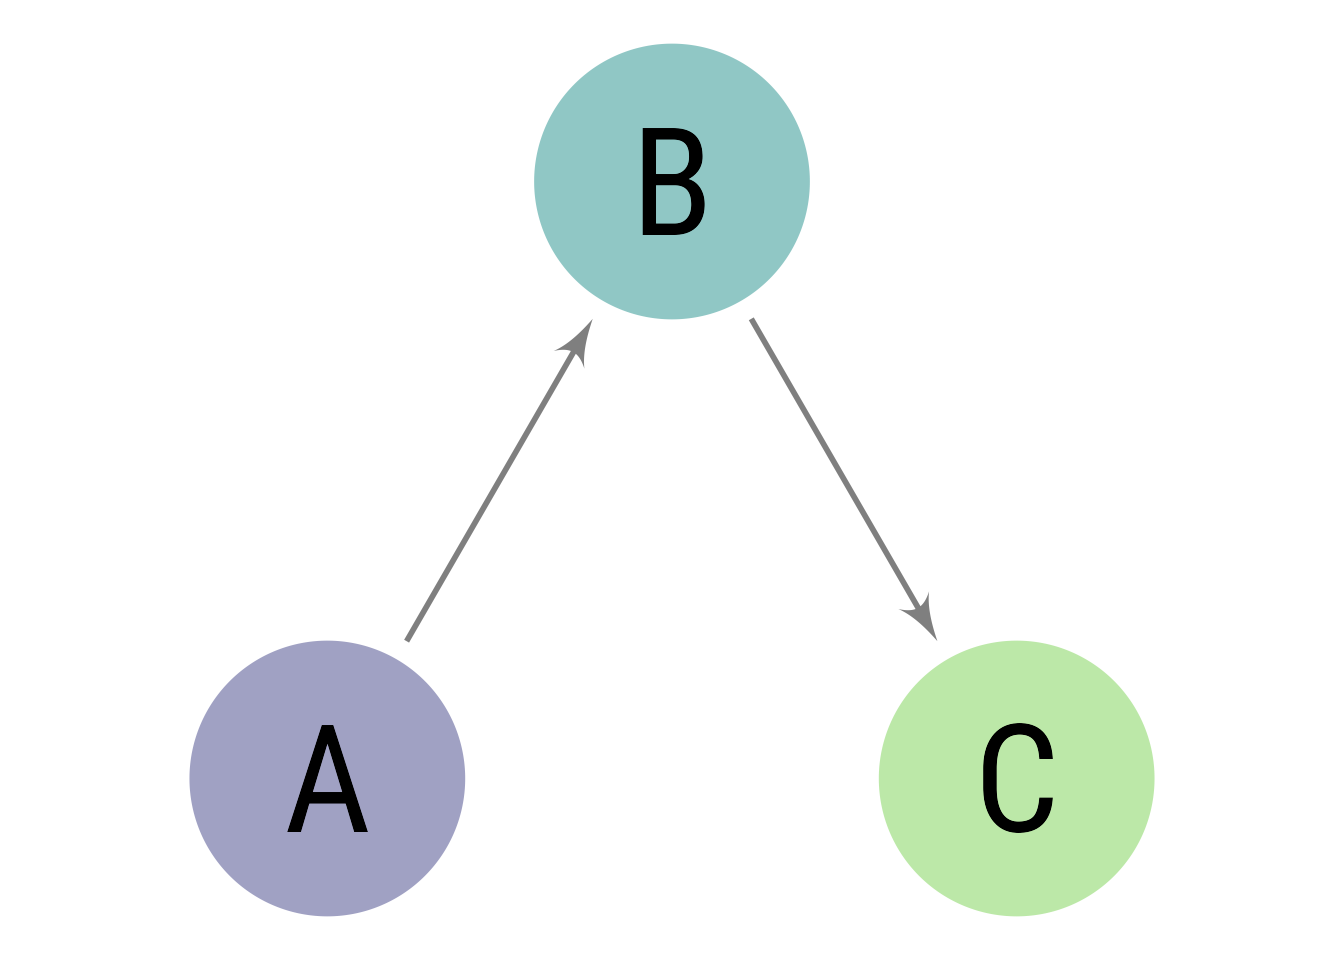
\includegraphics[width=1\textwidth,height=\textheight]{img/sampleimage.png}

{\noindent \emph{Note.} A note below the figure}

\end{figure*}

Figure graphics can be imported directly with Markdown:

\begin{figure}[!htbp]

{\caption{{Another Way to Import Graphics}{\label{fig-import2}}}}

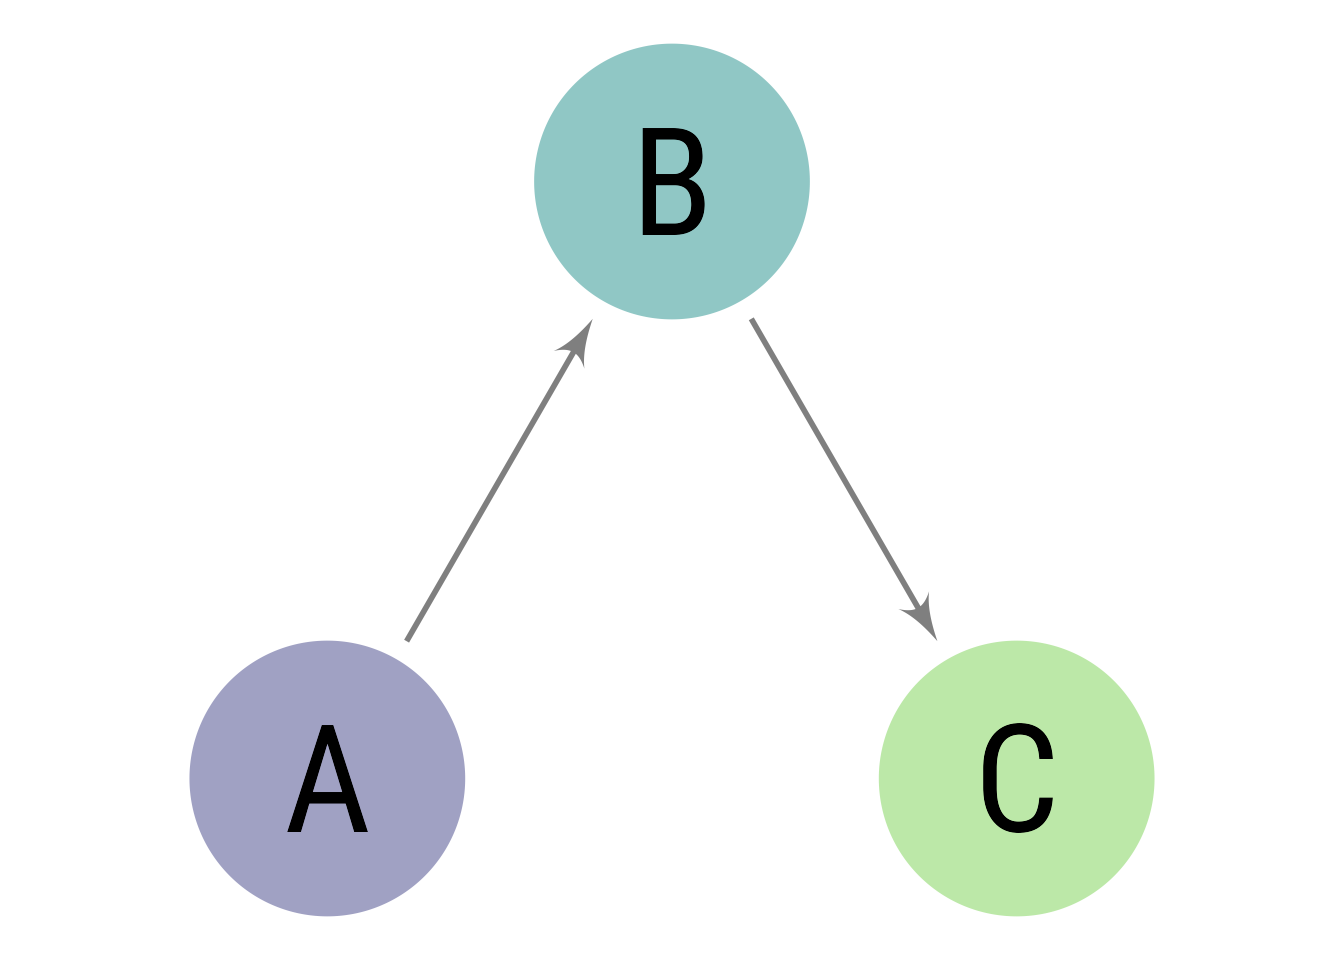
\includegraphics{img/sampleimage.png}

{\noindent \emph{Note.} A note below the figure}

\end{figure}

\subsection{Displaying Tables}\label{displaying-tables}

We can make a table the same way as a figure. Generating a table that
conforms to APA format in all document formats can be tricky. When the
table is simple, the \texttt{kable} function from knitr works well. Feel
free to experiment with different methods, but I have found that David
Gohel's \href{https://davidgohel.github.io/flextable/}{flextable} to be
the best option when I need something more complex.

\begin{ThreePartTable}

\global\setlength{\Oldarrayrulewidth}{\arrayrulewidth}

\global\setlength{\Oldtabcolsep}{\tabcolsep}

\setlength{\tabcolsep}{2pt}

\renewcommand*{\arraystretch}{1.5}



\providecommand{\ascline}[3]{\noalign{\global\arrayrulewidth #1}\arrayrulecolor[HTML]{#2}\cline{#3}}

\begin{longtable}[l]{|p{0.75in}|p{0.75in}}

\caption{\label{tbl-mytable}The Table Caption}

\tabularnewline

\ascline{0.75pt}{000000}{1-2}

\multicolumn{1}{>{\centering}m{\dimexpr 0.75in+0\tabcolsep}}{\textcolor[HTML]{000000}{\fontsize{11}{11}\selectfont{Numbers}}} & \multicolumn{1}{>{\centering}m{\dimexpr 0.75in+0\tabcolsep}}{\textcolor[HTML]{000000}{\fontsize{11}{11}\selectfont{Letters}}} \\

\ascline{0.75pt}{000000}{1-2}\endfirsthead 

\ascline{0.75pt}{000000}{1-2}

\multicolumn{1}{>{\centering}m{\dimexpr 0.75in+0\tabcolsep}}{\textcolor[HTML]{000000}{\fontsize{11}{11}\selectfont{Numbers}}} & \multicolumn{1}{>{\centering}m{\dimexpr 0.75in+0\tabcolsep}}{\textcolor[HTML]{000000}{\fontsize{11}{11}\selectfont{Letters}}} \\

\ascline{0.75pt}{000000}{1-2}\endhead



\multicolumn{1}{>{\centering}m{\dimexpr 0.75in+0\tabcolsep}}{\textcolor[HTML]{000000}{\fontsize{11}{11}\selectfont{1}}} & \multicolumn{1}{>{\centering}m{\dimexpr 0.75in+0\tabcolsep}}{\textcolor[HTML]{000000}{\fontsize{11}{11}\selectfont{A}}} \\





\multicolumn{1}{>{\centering}m{\dimexpr 0.75in+0\tabcolsep}}{\textcolor[HTML]{000000}{\fontsize{11}{11}\selectfont{2}}} & \multicolumn{1}{>{\centering}m{\dimexpr 0.75in+0\tabcolsep}}{\textcolor[HTML]{000000}{\fontsize{11}{11}\selectfont{B}}} \\





\multicolumn{1}{>{\centering}m{\dimexpr 0.75in+0\tabcolsep}}{\textcolor[HTML]{000000}{\fontsize{11}{11}\selectfont{3}}} & \multicolumn{1}{>{\centering}m{\dimexpr 0.75in+0\tabcolsep}}{\textcolor[HTML]{000000}{\fontsize{11}{11}\selectfont{C}}} \\





\multicolumn{1}{>{\centering}m{\dimexpr 0.75in+0\tabcolsep}}{\textcolor[HTML]{000000}{\fontsize{11}{11}\selectfont{4}}} & \multicolumn{1}{>{\centering}m{\dimexpr 0.75in+0\tabcolsep}}{\textcolor[HTML]{000000}{\fontsize{11}{11}\selectfont{D}}} \\

\ascline{0.75pt}{000000}{1-2}


\end{longtable}

\arrayrulecolor[HTML]{000000}

\global\setlength{\arrayrulewidth}{\Oldarrayrulewidth}

\global\setlength{\tabcolsep}{\Oldtabcolsep}

\renewcommand*{\arraystretch}{1}

{\noindent \emph{Note.} The note below the table.}

\end{ThreePartTable}

To refer to this table in text, use the \texttt{@} symbol followed by
the reference label like so: As seen in Table~\ref{tbl-mytable}, the
first few numbers and letters of the alphabet are displayed.

In Table~\ref{tbl-mymarkdowntable}, there is an example of a plain
markdown table with a note below it.

\begin{ThreePartTable}

\begin{longtable}[]{@{}llrc@{}}
\caption{Table Caption of a Markdown
Table}\label{tbl-mymarkdowntable}\tabularnewline
\toprule\noalign{}
Default & Left & Right & Center \\
\midrule\noalign{}
\endfirsthead
\toprule\noalign{}
Default & Left & Right & Center \\
\midrule\noalign{}
\endhead
\bottomrule\noalign{}
\endlastfoot
12 & 12 & 12 & 12 \\
123 & 123 & 123 & 123 \\
1 & 1 & 1 & 1 \\
\end{longtable}

{\noindent \emph{Note.} This is a note below the markdown table.}

\end{ThreePartTable}

What if you want the tables and figures to be at the end of the
document? In the .pdf format, you can set the \texttt{floatsintext}
option to false. For .html and .docx documents, there is not yet an
automatic way to put tables and figures at the end. You can, of course,
just put them all at the end, in order. The reference labels will work
no matter where they are in the text.

\subsection{Citations}\label{citations}

See
\href{https://quarto.org/docs/authoring/footnotes-and-citations.html}{here}
for instructions on setting up citations and references.

A parenthetical citation requires square brackets (Cameron \& Trivedi,
2013). This reference was in my bibliography file. An in-text citation
is done like so: Cameron and Trivedi (2013).

See
\href{https://wjschne.github.io/apaquarto/writing.html\#references}{here}
for explanations, examples, and citation features exclusive to apaquarto
like masked citations (citations masked for peer review) and possessive
citations (e.g., ``Schneider and McGrew's (2012) idea seemed reasonable
at the time.'')

\subsection{Masking Author Identity for Peer
Review}\label{masking-author-identity-for-peer-review}

Setting \texttt{mask} to \texttt{true} will remove author names,
affiliations, and correspondence from the title page. Any references
listed in the \texttt{masked-citations} field will be masked as well.
See
\href{https://wjschne.github.io/apaquarto/writing.html\#masked-citations-for-anonymous-peer-review}{here}
for more information.

\subsection{Hypotheses, Aims, and
Objectives}\label{hypotheses-aims-and-objectives}

The last paragraph of the introduction usually states the specific
hypotheses of the study, often in a way that links them to the research
design.

\section{Method}\label{method}

General remarks on method. This paragraph is optional.

Not all papers require each of these sections. Edit them as needed.
Consult the \href{https://apastyle.apa.org/jars}{Journal Article
Reporting Standards} for what is needed for your type of article.

\subsection{Participants}\label{participants}

Who are they? How were they recruited? Report criteria for participant
inclusion and exclusion. Perhaps some basic demographic stats are in
order. A table is a great way to avoid repetition in statistical
reporting.

\subsection{Measures}\label{measures}

This section can also be titled \textbf{Materials} or
\textbf{Apparatus}. Whatever tools, equipment, or measurement devices
used in the study should be described.

\subsubsection{Measure A}\label{measure-a}

Describe Measure A.

\subsubsection{Measure B}\label{measure-b}

Describe Measure B.

\subsection{Procedure}\label{procedure}

What did participants do?

How are the data going to be analyzed?

\section{Results}\label{results-1}

\begin{longtable}[]{@{}lllll@{}}
\toprule\noalign{}
Measure & F & df & \emph{p} & Partial η\^{}2 \\
\midrule\noalign{}
\endhead
\bottomrule\noalign{}
\endlastfoot
Age X education & 0.95 & 17 & 0.517 & 0.06 \\
Age X income & 1.27 & 27 & 0.174 & 0.13 \\
Age X BMI & 1.76 & 8 & 0.086 & 0.05 \\
Age X body dissatisfaction & 1.00 & 11 & 0.446 & 0.04 \\
Age X industry role & 1.28 & 7 & 0.261 & 0.03 \\
\end{longtable}

Table Caption of a Markdown Table

\subsection{Descriptive Statistics}\label{descriptive-statistics}

Here we describe the basic characteristics of our primary variables.

\section{Discussion}\label{discussion}

Describe results in non-statistical terms.

\subsection{Limitations and Future
Directions}\label{limitations-and-future-directions}

Every study has limitations. Based on this study, some additional steps
might include\ldots{}

\subsection{Conclusion}\label{conclusion}

Let's sum this up.

\section{References}\label{references}

\phantomsection\label{refs}
\begin{CSLReferences}{1}{0}
\bibitem[\citeproctext]{ref-CameronTrivedi2013}
Cameron, A. C., \& Trivedi, P. K. (2013). \emph{Regression analysis of
count data} (2nd ed.). Cambridge University Press.
\url{https://doi.org/10.1017/CBO9781139013567}

\bibitem[\citeproctext]{ref-schneider2012cattell}
Schneider, W. J., \& McGrew, K. S. (2012). \emph{The
{Cattell-Horn-Carroll} model of intelligence.}

\end{CSLReferences}

\section{Appendix}\label{appendix}

If there are multiple appendices, label them with level 1 headings as
Appendix A, Appendix B, and so forth.





\end{document}
